\section{Related Work}

\subsection{\cite{LabelingLanguageLearning}: In-Situ Labeling for Augmented Reality Language Learning}
%Huynh-2019 In-Situ Labeling for Augmented Reality Language Learning.
\cite{LabelingLanguageLearning} schaffen ein Framework, mit dem die Lernmethode 'loci' in Augmented Reality umgesetzt und erweitert werden kann. Die Lernmethode beruht darauf, Gegenstände der Welt mit Notizen zu beschriften. 

Dafür wurde folgende automatische Real-Time Objekt Erkennung entwickelt:

Mithilfe von Image Based Object Detection werden Objekte auf RGB-Fotos der AR Umgebung erkannt. Diese Objekte werden dann in die 3D Szene der Umgebung übernommen. 

Die AR Brille hat zu wenig Rechenleistung, um Image Based Object Detection durchzuführen, daher wurde eine Server-Client Architektur aufgesetzt. Die Videokamera der AR Brille wird verwendet, um Bilder von der Umgebung aufzunehmen. Die einzelnen Frames werden an den Server geschickt. Dieser nutzt ein neuronales Netzwerk, um alle erkennbaren Objekte in dem Bild zu finden und mit Bounding Boxen zu lokalisieren.

Die ObjectDetection API von TensorFlow wird verwendet. Es findet mehrere Objekte in einem Foto in einer Analyse und gibt Bounding Boxen an. Die Objekterkennung soll in Real-Time durchgeführt werden. Um die Laufzeit dieser möglichst gering zu halten, wird die niedrigste Kameraauflösung mit 896x504 Pixel verwendet und die Fotos werden als JPEG komprimiert. Damit braucht die Analyse 30 ms pro Foto. Dies ermöglicht eine Real-Time Erkennung mit 30 Frames pro Sekunde. 

Trotzdem ist die Erkennung in der Applikation durch einen Netzwerk Delay von 150 ms zwischen der Hololens und dem Server verspätet.

Die Hololens nummeriert die Frames, die an den Server geschickt werden. Zusätzlich wird für jedes Frame die Kameraposition gespeichert, mit der es aufgenommen wurde. So können Frames asynchron analysiert werden. 

Ist die Analyse durchgelaufen, werden die Bounding Boxen der Objekte und die Kameraposition genutzt, um die Objekte in der 3D Umgebung zu lokalisieren. Dafür wird der Mittelpunkt jeder Bounding Box mithilfe eines Raycastes in die 3D Szene projiziert.

Ein Objekt wird erst markiert, wenn es auf mehreren Fotos gefunden wurde, um Fehlern bei der Objekterkennung entgegenzuwirken. Durch die Analyse des ersten Fotos, wird eine ungefähre Position in der AR Umgebung für das Objekt ermittelt. Dieses Objekt wird dann mit den Objekten verglichen, die während der nächsten 60 Frames erkannt wurden. Haben die Objekte dieselbe semantische Bedeutung und eine ähnliche Position in der AR Umgebung, wird davon ausgegangen, dass es sich um ein einziges Objekt handelt, welches in den 60 Frames mehrmals aufgenommen wurde. 

Unser Vorgehen zur Objekterkennung ähnelt dem Framework von \cite{LabelingLanguageLearning}. Auch hier soll die AR Umgebung durch das Hinzufügen von Labels semantisch angereichert werden. Es wird ebenfalls ein neuronales Netz verwendet, um die Object Detection auf RGB-Bildern durchzuführen. Wir haben dafür keinen eigenen Server aufgesetzt, sondern nutzen einen Cloud Service von Microsoft Azure. Durch Abspeichern von erhobenen semantischen Informationen ist eine Real-Time Detektion nicht relevant. Daher kann die Bild-Analyse länger dauern, was es erlaubt, mehrere neuronale Netze zu verwenden, die nach unterschiedlichen semantischen Informationen suchen.

In Unserem Verfahren werden erkannte Objekte schon in der Umgebung markiert, wenn sie ein einziges mal erkannt wurden. Wenn das Objekt erneut aufgenommen wird, wird die neue Analyse dem Objekt die gleiche Klasse und eine ähnliche Position der AR Umgebung zuweisen. Daran lässt sich erkennen, das es sich um dasselbe Objekt handelt.

Die Erste Position die für das Objekt berechnet wurde und die Position, die aus der zweite Aufnahme hervorgeht, unterscheiden sich mit hoher Wahrscheinlichkeit ein wenig voneinander. Daher werden die Positionen gemittelt um eine akkuratere Position für das Label des Objektes zu finden. 
\citep{LabelingLanguageLearning}

\subsection{\cite{viewmanagement3d}: View Management for Virtual and Augmented Reality}

\cite{viewmanagement3d} beschreiben View Management für interaktive 3D Benutzeroberflächen. Als View Management wird die Positionierung von Labels bezeichnet.
Die Labels können sich auf eine 2D Ebene beschränken oder im 3D Raum liegen. View Management zielt darauf ab die Labels so zu positionieren, dass sie einander und relevante reale Objekte nicht verdecken. Gleichzeitig sollen die Labels die Gegenstände der Realen Welt auf eine verständliche Art annotieren. Labels sollen nahe bei den Objekten liegen, zu denen sie gehören.

Unsere Applikation würde durch View Management profitieren. Nachdem Gegenstände in der Umgebung erkannt wurden, werden sie in dem 3D Raum durch Labels markiert. Die Lesbarkeit dieser Labels kann durch View Management verbessert werden, indem ihre Positionen über Zeit verändert werden. 

Es müsste auf Veränderungen des Betrachtungswinkels und auf Hinzukommen von neuen Labels reagiert werden. Idealerweise würden die Labels einander und zusätzlich die Gegenstände der realen Welt nicht verdecken, die mit einem Label annotiert sind. 

View Management geht jedoch über den Rahmen dieser Arbeit hinaus und konnte nicht implementiert werden. \citep{viewmanagement3d}

\subsection{\cite{contextawaremixedreality}: Context-Aware Mixed Reality: A Framework for Ubiquitous Interaction}

\cite{contextawaremixedreality} stellen ein Framework vor, das einer AR Umgebung semantische Eigenschaften zuweist, um realistische Interaktionen zwischen virtuellen und realen Objekten zu erreichen. 
Insbesondere sollen physikalische Interaktionen an Realismus gewinnen.

Das Framework reichert die Umgebung mit Informationen über die Materialien an, aus denen reale Oberflächen und Gegenstände in der Umgebung bestehen. 
Die Umgebung wird in einer 3D Szene durch ein Mesh repräsentiert. Die einzelnen Voxel des Meshes werden mit Labels annotiert, um ihnen Semantik zuzuweisen.

Als beispielhafte Applikation wurde ein First-Person-Shooter vorgestellt, bei dem das Aussehen von Einschusslöchern davon abhängt auf welches Material geschossen wurde.

Für die Erkennung der Materialien werden mehrere Frames der Hololens segmentiert.
Die dadurch entstehenden semantischen Informationen werden abgespeichert, um bei späteren Interaktionen der AR Applikation abgerufen werden zu können. Die Erkennung der Materialien ist nicht echtzeitfähig, aber durch das Speichern der Materialien im Raum können die Interaktionen in Echtzeit ablaufen. Die Semantischen Informationen müssen nicht mit jedem Frame bestimmt werden.

RGB-Bilder der Umgebung werden aufgenommen und mit einem neuronalen Netzwerk analysiert, um semantische Informationen zu erheben. Das neuronale Netz wurde von \cite{contextawaremixedreality} für den First-Person-Shooter aufgesetzt. Das Netz wurde darauf trainiert 23 unterschiedliche Materialien zu erkennen und Bilder nach ihnen zu segmentieren. Dabei wird für jedes Pixel ein Material angegeben.

Mithilfe der Camera Position des Frames werden die Material-Informationen auf ein 3D Modell der Umgebung, ähnlich einer Textur, projiziert. Als Resultat wird an jedes Voxel des 3D Modells ein Label pro Frame gehängt, das die semantische Information wiedergibt, die in dem Frame erkannt wurde.

Bei der Segmentierung können Fehler auftreten, bei denen das auf dem Foto erkannte Material nicht dem realen Material entspricht. Um diesen Fehlern entgegenzuwirken werden mehrere Frames aufgenommen und analysiert. %Bildbereich, die schwer einzuordnen sind, werden in unterschiedlichen Frames unterschiedlich segmentiert. 

Die Informationen aus den Frames bilden sich auf die Voxel ab. Durch die Kumulierung der Segmentierungen erhält jedes Voxel eine Menge an Labels. Voxel die in schwer einzuordnenden Bildbereichen liegen, erhalten Labels die unterschiedliche Informationen beinhalten.

Um sicherzustellen, das jedes Voxel des 3D Modells nur eine semantische Bedeutung hat, werden die gesetzten Labels mit einer Baysian Fusion und einem neuronalen Netz überarbeitet. Als Resultat hat jedes Voxel nur ein einziges Label.

User Verfahren versucht ebenfalls das Verständnis der AR Umgebung durch semantische Informationen zu erweitern. Auch Wir nutzen ein neuronales Netzwerk um RGB-Fotos der Umgebung zu analysieren.
In unserem Verfahren erhält nicht jeder Pixel semantische Informationen, sonder nur Pixel, die die Position eines Gegenstandes markieren. Daher haben nur ausgewählte Voxel des 3D Meshes ein Label.\citep{contextawaremixedreality}

\newpage
\section{Grundlagen}
\subsection{Grundlagen zu Augmented Reality}
\subsubsection{Augmented Reality} %Einfürhung in AR

Augmented Reality vermischt die reale Welt mit digitalen (virtuellen) Elementen, um dem Nutzer eine erweiterte Wahrnehmung zu ermöglichen. Es können 3D Objekte, 2D Overlays oder Audioelemente verwendet werden um eine reale Umgebung mit Informationen zu bereichern. 

Die Umgebung beinhaltet den Teil der realen Welt, der in Augmented Reality abgebildet und erweitert werden soll. Beispielweise ein Zimmer, in dem eine AR Anwendung ausgeführt wird.
Die AR Umgebung umfasst die reale Umgebung und die virtuellen Elemente.

Augmented Reality weist drei grundlegende Merkmale auf: 
\begin{itemize}
	\item Die Realität wird mit dem Virtuellen kombiniert. Sie besteht darin, das die Realität mit virtuellen Elementen überlagert wird.
	\item Interaktion mit virtuellen Elementen erfolgen in Echtzeit.
	\item Virtuelle Elemente haben einen festen räumlichen Platz in der AR Umgebung.
\end{itemize}

Die Merkmal unterstützen ein möglichst nahtloses verschmelzen der realen Welt mit den virtuellen Elementen.

In einer AR Umgebung kann navigiert werden, indem der Nutzer sich physikalisch durch die reale Umgebung bewegt. Die reale Umgebung und die virtuellen Elemente stehen immer in dem gleichen räumlichen Verhältnis zueinander. Für AR ist keine andere Art der Navigation möglich, da sie die Verschmelzung der realen Welt und den digitalen Elementen brechen würden.

Da die reale Welt immer zu sehen ist, gibt sie eine Referenz und einen Kontext für die virtuellen Objekte an. 
Beispielsweise steht die Größe von virtuellen Objekten immer in Relation zu der realen Umgebung.\citep{GrundlagenAR}
%BookVirutalReality chapter 1

%müssen Informationen über die Umgebung erfasst werden. %Es ist wichtig zu bestimmen welche Objekte sich in der Umgebung befinden, die durch AR erweitert werden soll.

\subsubsection{AR System}

Ein AR System besteht aus der Hardware und Software, die benötigt wird um eine AR Umgebung zu erzeugen.

Das System muss die Vermischung der realen Welt mit virtuellen Elementen anzeigen und Interaktionen des Nutzers mit virtuellen Elementen, sowie Interaktion von virtuellen Elementen mit der realen Welt simulieren

Ein AR System ist in der Regel nicht an einen bestimmten Ort gebunden. Es kann in unterschiedlichen Umgebungen eingesetzt werden, die unterschiedliche reale Gegenstände aufweisen. AR Applikationen müssen diese unterstützen.\citep{GrundlagenAR}

%book Virutal reality chapter 1

\subsubsection{Grundlagen zu 3D Szenen für AR}


%todo was ist ein raycast?
%todo add something about szene graph

Die Virtuellen Inhalte der AR Anwendung werde in einer einer Virtuellen Szene gespeichert. 
AR Anwendungen müssen in Echtzeit laufen. Daher muss die Virtuelle Szene echtzeitfähig sein.
Im besten Fall kann ein Nutzer kein Unterschied zwischen der virtuellen Welt und der realen Welt, bezüglich auf zeitliche Verzögerungen, bemerken.

Um Interaktion mit digitalen Elementen zu ermöglichen, werden relevante Teile der realen Welt in der 3D Szene repräsentiert. 
So werden beispielsweise die Wände und der Boden eines Raumes in der Szene abgebildet. Auch die Position eines Controllers und die Blickrichtung des Nutzers kann mit Sensoren verfolgt und in die Szene miteinbezogen werden.

\subsubsection{Spatial Mapping} 
Um virtuelle Objekte an eine Umgebung anzupassen und Interaktion zwischen virtuellen Objekten und der realen Umgebung zu ermöglichen, benötigt ein AR System Informationen über die Geometrie der Umgebung.

Mit den Sensoren der AR Hardware werden Informationen gesammelt, die Aussagen über die Geometrie der Umgebung treffen. Beispielsweise haben AR Geräte eine Tiefenkamera, die Entfernung messen kann. Die Daten der Sensoren werden gesammelt und in Relation zu der Bewegung des Gerätes gesetzt um die Umgebung zu Rekonstruieren. Dieser Vorgang nennt sich Spatial Mapping. 

Mit der Entstehenden Spatial Map können digitale Elemente mit der Umgebung interagieren, diese verdecken oder von ihr verdeckt werden.\citep{spatialMapping} 

\begin{figure}[H]
	\centering
	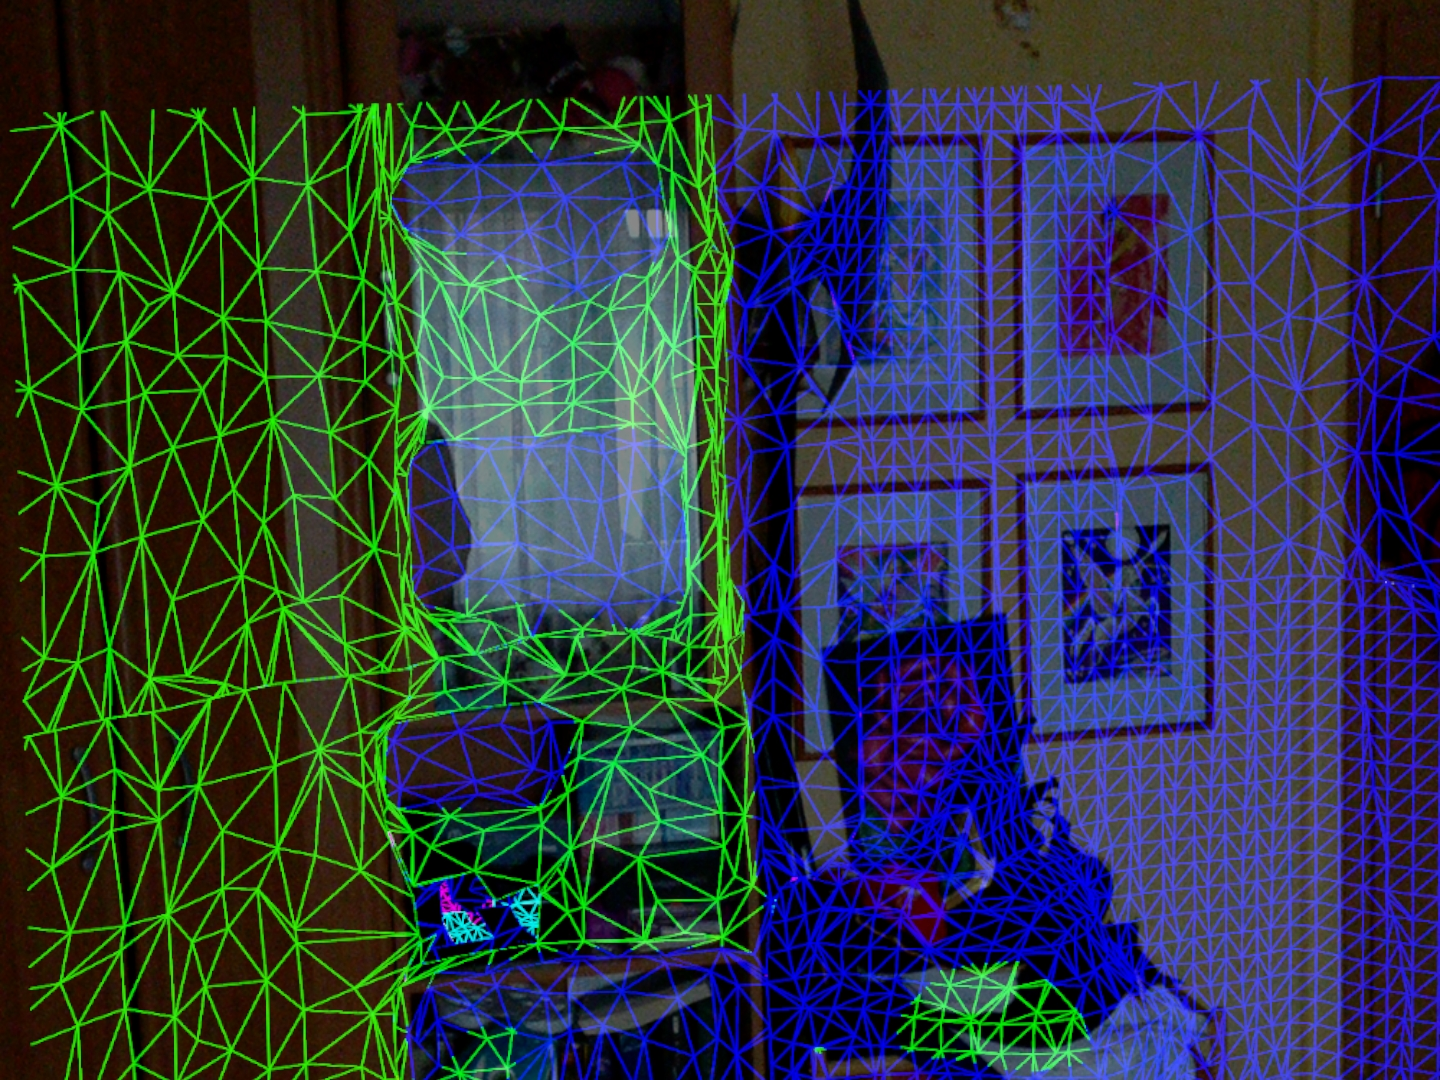
\includegraphics[width=0.7\textwidth]{images/ML_20201003_15.36.42.jpg}
	\caption[]{Spatial Map}
	\label{img:spatialmap}
\end{figure}

\subsubsection{View Management}

%\cite{viewmanagement3d} beschreiben View Management für interaktive 3D Benutzeroberflächen. Als View Management wird die Positionierung von Labels bezeichnet.
%Die Labels können sich auf eine 2D Ebene beschränken oder im 3D Raum liegen. View Management zielt darauf ab die Labels so zu positionieren, dass sie einander und relevante reale Objekte nicht verdecken. Gleichzeitig sollen die Labels die Gegenstände der Realen Welt auf eine verständliche Art annotieren. Labels sollen nahe bei den Objekten liegen, zu denen sie gehören.
%
%Unsere Applikation würde durch View Management profitieren. Nachdem Gegenstände in der Umgebung erkannt wurden, werden sie in dem 3D Raum durch Labels markiert. Die Lesbarkeit dieser Labels kann durch View Management verbessert werden, indem ihre Positionen über Zeit verändert werden. 
%
%Es müsste auf Veränderungen des Betrachtungswinkels und auf Hinzukommen von neuen Labels reagiert werden. Idealerweise würden die Labels einander und zusätzlich die Gegenstände der realen Welt nicht verdecken, die mit einem Label annotiert sind. 
%
%View Management geht jedoch über den Rahmen dieser Arbeit hinaus und konnte nicht implementiert werden. \citep{viewmanagement3d}


Die virtuellen Informationen die einen Teil der realen Welt bereichern, werden meistens als 3D Elemente angezeigt. 
Die Informationen kann jedoch auch in 2D Elementen angezeigt werden, die sich auf eine 2D Ebene beschränkt. Insbesondere Labels, die reale Objekte erklären, können auf diese Art angezeigt werden.

Das Layout der 2D Elemente auf der Ebene wird durch View Management optimiert.
Idealerweise werden die Elemente so positioniert, das sie sich Gegenseitig nicht verdecken, relevante Bereiche der realen Welt nicht verdecken.
Zusätzlich sollen sie nah an den Gegenständen der Realen Welt bleiben, die sie annotieren. Siehe Abbildung \ref{viewManagement}.

\begin{figure}[H]
	\centering
	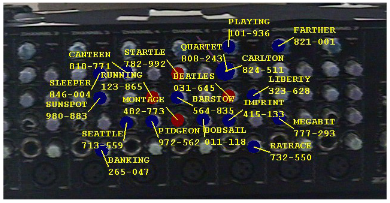
\includegraphics[width=0.7\textwidth]{images/ViewManagementImageFromPaper.PNG}
	\caption[]{Labels durch View Management positioniert.\citep{viewmanagement}}
	\label{viewManagement}
\end{figure}
Das Layout muss angepasst werden, wenn sich der View verändert. Gleichzeitig soll das Layout stabil bleiben und sich nicht verändern, wenn ein Anderes Layout ein wenig besser wäre, um ein hin und her springen zwischen zwei möglichen Layouts zu vermeiden.\citep{viewmanagement}

%todo rework this a little

\subsection{Magic Leap AR Brille}

Die Magic Leap One Lightwear ist eine Augmented Reality Brille, die von dem Unternehmen Magic Leap entwickelt wurde. Sie verfügt über ein Head-Mounted Display und einer Recheneinheit die über ein Kabel mit dem Display verbunden ist. Die Recheneinheit kann an der Hüfte getragen werden, was die AR Brille Mobil macht. 


\subsubsection{Hardware}

Die Recheneinheit besitzt zwei Denver 2.0 64 Bit Prozessor-Kerne und vier ARM Contex A57 46 bit Kerne. Davon ist einer der Denver Kerne und zwei der ARM Contex Kerne für Applikationen nutzbar.  

Sie besitzt neun Sensoren und mehrere Kameras. Dazu gehören:
\begin{itemize}
	\item ein Infrarot Tiefen-Sensor,
	\item ein Eye Tracker,
	\item eine Foto und Video Kamera, die im Format 16:9 mit einer Auflösung von 1920 x 1080 Pixeln aufnehmen und
	\item mehrere Umgebungskameras die in unterschiedliche Richtungen ausgerichtet sind. \citep{mlofficialsalespitch,mlglossary}
\end{itemize}

Der Output geschieht über ein Display mit einem 50 Grad Field of View und einem Seitenverhältnis von 4:3. Das Display ist transparent. Daher kann die reale Welt immer betrachtet werden. Selbst wenn ein weißes Objekt angezeigt wird, schimmert die reale Welt noch durch. 
Das Display kann keine Schwarzen Objekte anzeigen. 

Eingaben erfolgen über einen 6 Degree of Freedom Controller. Er verfügt über 3 Knöpfe (Trigger, Bumper, Home Button) und ein Touchpad. \citep{mlofficialsalespitch,mlglossary}

\begin{figure}[H]
	\centering
	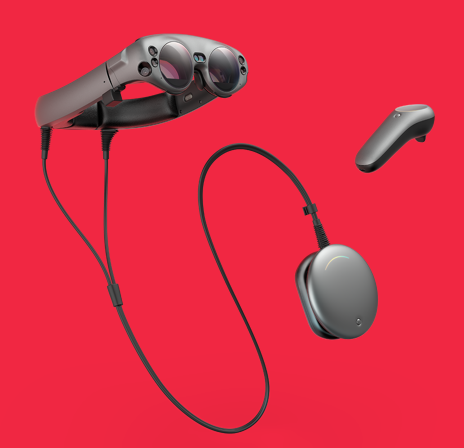
\includegraphics[width=0.7\textwidth]{images/img_magicLeap.PNG}
	\caption[]{Magic Leap One AR Brille.\citep{mlImage}}
	\label{viewManagement}
\end{figure}

\subsubsection{Betiebssystem}
Die Magic Leap Brille läuft auf dem Betriebssystem Lumin OS. Dieses wurde für Augmented Reality entwickelt und bietet Applikationen entsprechende Funktionalitäten an. Beispielsweise führt das Betriebssystem Spatial Mapping durch.\citep{mlluminOS,mlluminfeatures}

Dabei werden mit den Sensoren und Kameras der Brille Daten aufgenommen und in einen zeitlichen Zusammenhang mit der Bewegung der Brille gesetzt, um eine Rekonstruktion des Raumes zu erhalten.\citep{mlluminOS,mlluminfeatures,mlluminworldreconstruktion,mlmeshingunity}

Lumin OS bietet es Applikationen an,
\begin{itemize}
	\item Raycasts auf die Umgebung durchzuführen und
	\item ein Mesh der Rekonstruktion zu erhalten.
\end{itemize}
Neben dem Spatial Mapping unterstützt Lumin OS das Verarbeiten vom Input des Controllers und verwaltet die Zugriffsrechte der Applikationen. Dazu gehört beispielsweise das Recht (Permission) die Fotokamera und das Netzwerk zu nutzen.\citep{mlluminfeatures,mlappsecurity}

Selbst wenn mehrere Applikationen das recht dazu haben, kann nur eine Applikation zum gleichen Zeitpunkt auf die Fotokamera zugreifen. Die Applikationen müssen sich mit der Kamera-Ressource von Lumin 0S verbinden, diese reguliert, welche Applikation Foto-Anfragen stellen kann und die Aufgenommenen Fotos erhält. 


%MLCamera greift auf die Foto-Kamera zu. Über dieses Skript kann die Applikation sich mit der Kamera-Ressource verbinden. Nur eine Applikation kann mit der Kamera verbunden sein. Nur die verbundene Applikation kann Foto-Anfragen stellen und Aufgenommene Fotos erhalten. Anfragen und Resultatdaten werden ebenfalls durch MLCamera behandelt.

Es können niemals mehrere Applikationen zugriff auf die physikalische Kamera der Magic Leap One haben. Kamera Ressource
Permission stufen

\subsubsection{Unity Applikationen für Magic Leap One}
%
Unity ist ein eine Entwicklungsumgebung, mit der Applikationen für Lumin OS erstellt werden können. Ein Unity Projekt besteht aus mindestens einer Szene, in der mehrere GameObjects exsiteren. 'GameObject' ist ein Oberbegriff für alle Elemente, die in der Szene existieren. Sie bilden eine Heirarchische Strukur, in der GameObjects Parents und Children anderen GameObjects sind.\citep{unitygameobject}

GameObjects haben in sich keine Funktionalität und kein Aussehen. Diese werden durch Components hinzugefügt. Einige Components sind bereits in Unity integriert. Sie geben einem GameObject eine Position in der Szene (Transform Component), machen sie Sichtbar (Mesh Renderer) und führen alle sonstige Programmlogik durch, die notwendig ist. Um eine neue Funktionalitäten zu implementieren, kann ein C\# Script geschrieben werden und einem GameObject als Component zugewiesen werden.

Magic Leap unterstützt die Entwicklung von Applikationen für Lumin OS mit Unity. Ein Unity Project Template von Magic Leap erleichtert das Set up der Applikation. Dazu gehören Build Optionen und das Einstellen der Haupt Kamera der Szene - der Unity Kamera. Die Unity Kamera rendert die Szene für das Display der Magic Leap One. Die Kamera verfolgt die Bewegung der Magic Leap Brille und kopiert diese in der Unity Szene. %Die Szene bleibt somit stationär und die Kamera bewegt sich in ihr, so wie der Nutzer der Magic Leap sich in einer Umgebung bewegt.

Das Unity Template verfügt über vorgefertigte Skripts, die auf Funktionalitäten von Lumin OS zugreifen:

\begin{itemize}
	\item MLInput stellt Informationen über den Controller zur Verfügung. Damit können die Knöpfe und Touchpad-Gesten überwacht werden.
	\item MLCamera greift auf die Foto-Kamera zu. Foto-Anfragen und Resultatdaten werden ebenfalls durch MLCamera behandelt.
	\item MLPrivilegeRequestBehavior ermöglicht es den Nutzer um das Recht zu Fragen, auf bestimmte Teile des AR Systems zuzugreifen. Beispielsweise muss nach Permission gefragt werden, um die Foto-Kamera Ressource zu verwenden. 
	\item MLRaycast greift auf die Spatial Mapping Funktionalitäten von Lumin OS zu. Es frage das Betriebssystem darum, einen Raycast auf die Rekonstruktion der Umgebung durchzuführen. 
	\item MLSpatialMapper zeigt Rekonstruktion der Umgebung von Lumin OS als Mesh an. Das Mesh besteht aus GameObjects, die von MLSpatialMapper erzeugt werden. Sie werden ständig aktualisiert, um das geometrische Verständnis von Lumin OS widerzuspiegeln.
\end{itemize}

Scripts können von der Klasse Monobehavior erben. Monobehaviors verfügen über Methoden, die von Unity zu unterschiedlichen Events der Laufzeit ausgeführt werden. Nur Skripts die ein Component eines GameObjects sind, werden aufgerufen.

\begin{itemize}
	\item Awake - Diese Methode wird aufgerufen, wenn das GameObject initialisiert wird. %Wenn ein GameObject initialisiert wird, werden die Awake() Methoden der Componenten aufgerufen.
	\item Update - Die Update Methoden der Scripts werden zu jedem Frame aufgerufen.
	\item OnDestory - Diese Methode wird aufgerufen, wenn das GameObject aus der Szene gelöscht wird.
\end{itemize}

Monobehaviors können über Globale Variablen verfügen. Wenn das Skript einem GameObject als angehören, kann der Inhalt der Globalen Variable in Unity modifiziert werden. Dadurch kann einem Skript eine Referenz auf ein bestimmtes GameObject gegeben werden. %todo show this one?

Monobehaviors können als Singleton fungieren, indem sie eine globale statische Referenz auf sich selber anlegen, wenn ihre Awake Methode aufgerufen wird. Dadurch kann jedes andere Script, die Instanz des Singletons aufrufen, indem sie die statische Referenz der Klasse des Singletons verwenden %auf die instanz der  ohne aufwändig nach dem Component zu suchen in dem es sich befindet. durch die Instanz durch die Referenz auf die Instanz des Singletons, auf das Singleton zugreifen.
%todo add code examples of this I guess.
%todo gmaobjects have lokal koordinatensystem. szene has global. unity camera has camera space
Skripts können während der Laufzeit GameObjects erzeugen. Um festzulegen, wie das GameObject aussehen soll, kann in dem Unity Editor ein Prefab erstellt werden. Ein Prefab ist ein vorgefertigtes, Abgespeichertes GameObjekt, dessen Child Objects, Components und globalen Variablen der Components werden festgelegt werden. Das Prefab fungiert als Vorlage für GameObjects die zur Run Time initialisiert werden.

Währen der Initialisierung wird die Position in dem globalen Koordinatensystem für das neue GameObject angegeben werden. Nachdem das Objekt initialisiert wurde, kann auf seine Components und Scripts zugegriffen werden.\citep{unityprefabs}


\subsubsection{Lokale und globale Koordinatensysteme in 3D Szenen}
%\newline
In einer 3D Szenen werden die Positionen von Objekten als Matrizen in dreidimensionalen Koordinatensystemen verwaltet.
Es gibt ein globales Koordinatensystem (auch Weltkoordinatensystem oder World Space), in dem alle Objekte relativ zu einem gewählten Ursprung liegen. 

Jedes Objekt hat zusätzlich ein eigenes, lokales Koordinatensystem (Objektkoordinatensystem). Dessen Ursprung liegt in dem jeweiligen Objekt.
Die Position und Rotation des Objektes in dem globalen Koordinatensystem bestimmt die Relation zwischen dem globalen und dem lokalen Koordinatensystem. 

Das lokale Koordinatensystem einer Kamera wird auch Camera Space genannt. Die Relation zwischen dem Camera Space und dem globalen Koordinatensystem wird in Unity durch die cameraToWorld Matrix beschrieben. Mithilfe dieser Matrix kann eine Koordinate aus dem Camera Space in die entsprechende Koordinate des globalen Koordinatensystems transformiert werden.\citep{unitycameratoworldmatrix}

Dazu wird die Koordinate als Vektor angegeben und mit der cameraToWorld Matrix multipliziert. Das Resultat ist ein Vektor, der eine Koordinate im globalen Koordinatensystem angibt.\citep{unitycameratoworldmatrix,unitymultiplyoint}

\subsubsection{Kamera in 3D-Computergrafik}
\paragraph{View Frustum}
ist das Teilvolumen einer 3D Szene, die auf den zweidimensionalen Bildschirm abgebildet wird. Alle Objekte die von der Kamera gesehen werden, befinden sich in dem View Frustum.

\paragraph{Clipping Plane}
bezeichnet eine Ebene, die den View Frustum quer zur Blickrichtung begrenzt. 
Es gibt eine vordere und eine hintere Clipping Plane.
Die vordere Clipping Plane liegt nah an der Kamera. Alle Objekte die zwischen der Kamera und der vorderen Clipping Plane liegen, werden nicht angezeigt.

Die hintere Clipping Plane limitiert wie weit Objekte entfernt sein können, bevor sie nicht mehr zu sehen sind.

%to myself: yay :) you're doing well I believe in you!

\subsection{Computer Vision}
Computer Vision setzt das Ziel die Inhalte digitaler Bilder und Videos zu verstehen. Sowohl semantische als auch geometrische Inhalte werden dabei analysiert. 

Im diesem Feld kommen Statistik, Bilderverarbeitung und Maschinelles Lernen zum Einsatz. Maschinelles Lernen  um neuronale Netze zu formen, die Bild und Video Analysen durchführen können. Diese Netze müssen mit großen Mengen an Beispieldaten Trainiert werden und können dann, Aufgaben, wie Objekterkennung, Menschen Erkennen und Bewegungen in Videos Nachverfolgen.\citep{intortodeeplearingmedical}

Maschine Learning ist darauf ausgelegt eine automatische Entscheidung über einen Gegebenen Datensatz zu treffen. In einer Trainings Phase In Computer Vision wird maschine learning besteht die aufgabe generell darin eine automatische Entscheidung zu treffen. 


Eine Grundlegende Aufgabe ist das Image Classification. Die Aufgabe besteht darin eine automatische Entscheidung zu treffen
%what is deep learning?
%Deep Learing 
%
%Machine Learning trifft eine automatische Entscheidungen. Beispielweise zwischen apfel und birne
%Training Phase. Mit TrainigsDaten die vorbereitet sind und bedeutende features extrahiert sind.
%vorbereitet durch preprocessing mathoden. Dabei werden Bilder verändert um beispielsweise rauschen zu entfernen. Die Form der Daten bleibt gleich. Das Resultat von Preprocessing ist ein Bild.
%Freature extracion ist die aufgabe einen algorithmus zu erstellen, der eine eindeutige und komplete preräsnetnation eines features aus den Eingabedaten erheben kann. 
%
%Feature Extracion lässt sich nicht generealisieren. Für jede Applikation muss ein neues set and Traingsdaten erstellt werden, wobei die features die in den Daten erkannt werden sollen per hand angegeben werden. ein neuer feature Extraktion algorithmus entworfen werden. 
%
%Ein Algorithmus wird  

%Image Segmentation
%
%Bei der Image Classification wird ein Bild mit einem Objekt als Input gegeben. Die aufgebae gesteht darin die Klasse oder den Typ des Objektes zu bestimmen.
%
%Objekt Localization 
%
%Die Typen or der Klassen von Objekten in einem Bild finden. 
%
%Der Input ist ein Bild mit einem einzigen Objekt.
%Der Output identifiziert die klassen. 

%todo more about this



\subsubsection{Object Detection}
Image Based Object detection reinbauen :)

Objekt Detection ist eine Aufgabe der Computer Vision. Es sollen mehrere Objekte in einem Bild erkannt werden. Spezialisierungen von Object Detection sind beispielsweise Gesichtserkennung oder Fußgänger erkennen. Durch eine Objekterkennung werden semantische Inhalte eines Bildes automatisch erhoben. 

Für die Objekte wird eine Klasse und eine Bounding Box bestimmt. 
Die Klasse gibt an, um welche Art von Objekt es sich handeln. Beispielsweise ob es eine Tastatur oder ein Computerbildschirm ist. (Object classification)
Die Bounding Box gibt ein Viereck in dem Bild an, in dem sich das Objekt befindet.(object localization)

Object Detection besteht aus drei 



%Object Detection Performance und Genauigkeit study
%vs 
%3d Basierte Detection
%todo more about this

\subsubsection{Artificial Neural Networks}
Artificial Neural Networks sind Machine Learning Architekturen. Sie können beispielsweise Musik, Text oder Bilder nach Mustern durchsuchen. Sie sind für keine genaue Aufgabe programmiert, sondern lernen indem sie mit Beispieldaten trainiert werden. 

Für jedes Beispiel gibt es ein Label, das angibt ob es das gesuchte Muster enthält oder nicht. Die Struktur des Networks verfügt über Gewichte, die Einfluss auf den Output haben. Mit jedem Trainingsbeispiel passt das Network die Gewichte an, sodass der Output dem Label des Beispiels entspricht.\citep{introToCNN,surveyOfDeepLearing}

Artificial Neural Networks bestehen aus einer Menge an verbundenen Knoten, die jeweils eine Berechnung durchführen. Diese Knoten sind in Ebenen aufgeteilt, den Input Layer, den Output Layer, und mehrere Hidden Layer dazwischen. Die Knoten einer Ebene sind mit allen Knoten der Vorherigen Ebene verbunden.\citep{introToCNN,surveyOfDeepLearing}

Das Neural Network bekommt eine Menge an Daten als Input. Die Knoten arbeiten zusammen um den Output zu erzeugen. Dabei wird über Gewichte entschieden, wie viel Einfluss das Ergebnis der einzelnen Knoten auf die nächste Ebene hat.\citep{introToCNN,surveyOfDeepLearing}

Um ein Neural Network zu trainieren, wird der Output von einem Mensch bewertet. Das Neural Network nutzt diese Bewertung, um die Gewichte der einzelnen Knoten zu verändern. So passt sich das Neural Network an. \citep{introToCNN,surveyOfDeepLearing}

\subsubsection{Convolutional Neural Networks}
Convolutional Neural Networks sind auf das Verarbeiten von Bildern spezialisiert. Sie nutzen aus, das Bilder viele Redundanzen und informationsarme Bereiche haben. Daher können mit jedem Verarbeitungsschritt des Networks Informationen weggelassen werden. So können Rechenzeit und Volumen der Trainingsdaten verringert werden.\citep{introToCNN,surveyOfDeepLearing,cNNforClass}

Convolutional Neural Networks sind Machine Learning Architekturen, die darauf ausgelegt sind, Muster in Bildern zu erkennen. Sie müssen auf das Muster trainiert werden. Dazu wird ihnen eine Menge an Bildern, die Teilweise das Muster erhalten, und der gewünschte Output, der erreicht werden soll, gegeben. Die Struktur des Network verfügt über Gewichte, die die Berechnung des Outputs beeinflussen. Mit jedem Trainigsbild passt das Network die Gewichte an, damit es die Mustern korrekt erkennen kann.\citep{introToCNN,surveyOfDeepLearing}

Convolutional Neural Networks werden hauptsächlich eingesetzt um Muster in Bildern zu erkennen. Daher ist ihre Struktur und ihre Arbeitsweise auf Bilder spezialisiert. Sie brauchen weniger Rechenzeit und weniger Trainingsdaten als ein generelles Artificial Neural Network für dieselbe Aufgabe brauchen würde.\citep{introToCNN,surveyOfDeepLearing,cNNforClass} 

Die Knoten in einer Ebene eines Convolutional Neural Network sind nur mit wenigen Knoten der vorherigen Ebene verbunden. So sinkt die Menge an Informationen mit jeder Ebene. Das CNN wird gezwungen sich auf wesentliche Teile des Bildes zu konzentrieren, mit denen beispielsweise ein Objekt oder  Muster erkannt werden kann. \citep{introToCNN,surveyOfDeepLearing}

\subsubsection{Azure Computer Vision Services}

Über eine REST API erreichbar. 

Rest steht für Representational State Transfer. Eine Rest API ist eine Programmierschnittstelle die sich am dem Verhalten des world wide web orinetiert. Die Kommunikation zwischen einem client und dem server orientiert sich an REST.
Rest steht für Representation State Transfer und bezeichnet einen Architenkturansatz wie verteile Systeme miteinander kommunizieren können. REST verlangt unter anderem ein Client-Server Modell eine zustandslose Kommunikationen zwischen ihnen. Jede Anfrage eines Client beinhaltet alle Informationen die der Server benötigt um sie zu beantworten. %rest is just an idea. describe it a bit more

Eine Rest-Api kann mit http/s realisiert werden. Der Server / Service kann durch eine URL angespochen werden. Diese wird auch Endpoint genannt. HTTP-Methoden, wie GET und POST kommunizieren an den Service welche Operation durchgeführt werden soll. Diese werden auch Http-Anfragen oder HTTP Request genannt. Mit Get werden Daten von dem Server angefordert. Die Post Methode erlaubt das übermitteln von zusätzlichen Daten an der Server.

Aufbau eines HTTP Requests. Start Line. HTTP methode, get, put. endpoint url. http version die die strukutr der rest der nachricht definiert.
headers. in den headers können beispielsweise eine autentifizierung für die API sein.

Body. Manche HTTP Methoden, wie zum beispiels POST müssen dem Server Daten übertragen. diese werden in dem Body der Nachricht untergebracht.
  
Auf jede Http-Anfrage wird ein HTTP-Responsecode als Antwort zurückgeschickt. Mit dem Code wird dem client mitgetial, ob die anfrage erfolgreich bearbeitet wurde. Wenn ein Error aufgetreten ist, gibt der Statuscode Auskunft über die Art des Errors. 

Beispiel Responsecodes:
\begin{itemize}
	\item 404 - Url nicht gefunden
	\item 401 - Zugriff verweigert wegen ungültiger Authentifizierung
	\item 400 - Fehlerhafte Anfrage. Der Service konnte die Anfrage nicht verstehen
	\item 200 - Anfrage wurde erfolgreich bearbeitet
\end{itemize}

Eine API wird, bei einer erfolgreichen Bearbeitung der Anfrage in dem Körper der HTTP-Response die erfragten Daten mitschicken.
HTTP Response aufbau.
status line gibt den response code an, die protocol version und einen status text, der den response code erklären kann.
headers
body. abhänig von dem response code werden in der Response Daten übertragen. diese sind im Body.
Headers gegeben Art der Daten und Länge an.

%todo: make pretty

\subsubsection{Azure Object Detection}
Microsoft Azure bietet einen Computer Vision Service an. Dabei handelt es sich um mehrere KIs, die für unterschiedliche Aufgaben trainiert wurden. Dazu gehört unter anderem ein Service für Object Detection.

Dabei sendet der Anwender ein Bild an Microsoft, dort wird es verarbeitet und ein Ergebnis in Form einer Json Datei zurückgeschickt.\citep{getAzure,whatIsAzure,objDetectAzure,Azure302Doc}

Die Object Detection basiert auf einem trainierten KI Modell. Dieses kann nur Objekte erkennen, für die es trainiert wurde.
Zusätzlich können Objekte, die in dem Foto sehr klein sind oder nah bei anderen Objekten liegen, nicht erkannt werden.\citep{azureobjdetec}

Der Service ist durch eine REST-API erreichbar. Mit einer Post Anforderung werden die Bilddaten übertragen und die Analyse angefragt. Die Response Nachricht beinhaltet eine Json-Datei, welche die gefundene Objekte und deren Positionen auf dem Foto beinhaltet. 
Um den Service zu nutzen wird eine Http Post Anforderung an die WebAdresse geschickt. Als Endpoint wird die Web Adresse des der REST-API Angegeben. die Nachricht muss folgenden Inhalt haben:
\begin{itemize}
	\item Ein Authentifizierungs-schlüssel, der mit einem Azure Account verbunden ist
	\item und Bilddaten
\end{itemize}

Das Resultat der Analyse wird in der ResponseNachricht zurückgeschickt. Der Responsecode 200 gibt an, das die Analyse durchgeführt wurde. In diesem Falle wird eine Json Datei mitgeschickt. Beispielhaft:

\begin{lstlisting}
{"objects":[{"rectangle":{"x":1377,"y":900,"w":157,"h":138},"object":"computer mouse","confidence":0.681},
{"rectangle":{"x":1336,"y":0,"w":584,"h":841},"object":"display","confidence":0.873},
{"rectangle":{"x":315,"y":25,"w":906,"h":622},"object":"display","confidence":0.839},
{"rectangle":{"x":447,"y":800,"w":862,"h":166},"object":"computer keyboard","confidence":0.71}],
"requestId":"a77e261a-7d40-4159-bf78-19d8fb61ad92",
"metadata":{"height":1080,"width":1920,"format":"Jpeg"}}
\end{lstlisting}

Die gefundenen Objekte befinden sich in der Liste mit dem Key 'objects'. Jedes Element der Liste hat ein Bounding Box 'rectangle' und eine Klassenbezeichnung 'object'. Zusätzlich hat jedes Object einen 'confidence' Score. Dieser gibt die Wahrscheinlichkeit an, das das Objekt korrekt erkannt wurde. 
Neben den Objekten wird noch eine requestId und Metadaten über das Bild zurückgeschickt.

\subsubsection{Azure Custom Vision}
Azure bietet zusätzlich einen Computer Vision Service an, den der Nutzer trainieren kann. 
Das verwendete KI Modell ist für Objekt Detection entwickelt und ist nicht vor-trainiert.
Custom Vision kann dann verwendet werden, wenn Azure Object Detection für Objekte nicht trainiert ist.\citep{Azure302bDoc}

Das KI Modell lässt sich für Image Klassifizierung oder Objekt Detection trainieren. Über eine Webseite lässt sich der Trainingprozess des Modells steuern und auswerten. Der Nutzer lädt Fotos hoch und fügt jedem Foto händisch einen oder mehrere Tags hinzu. Die Tags geben die Objekt-Klasse an, die sich in dem Bild befindet. Um das Modell für Object Detection zu trainieren, kann eine rechteckige Region in dem Foto markiert werden, um das Objekt zu lokalisieren. Siehe Abbildung \ref{img:trainingone}. In einem Bild können mehrere Regionen markiert werden. Jede Region wird mit einem Tag annotiert.

\begin{figure}[H]
	\centering
	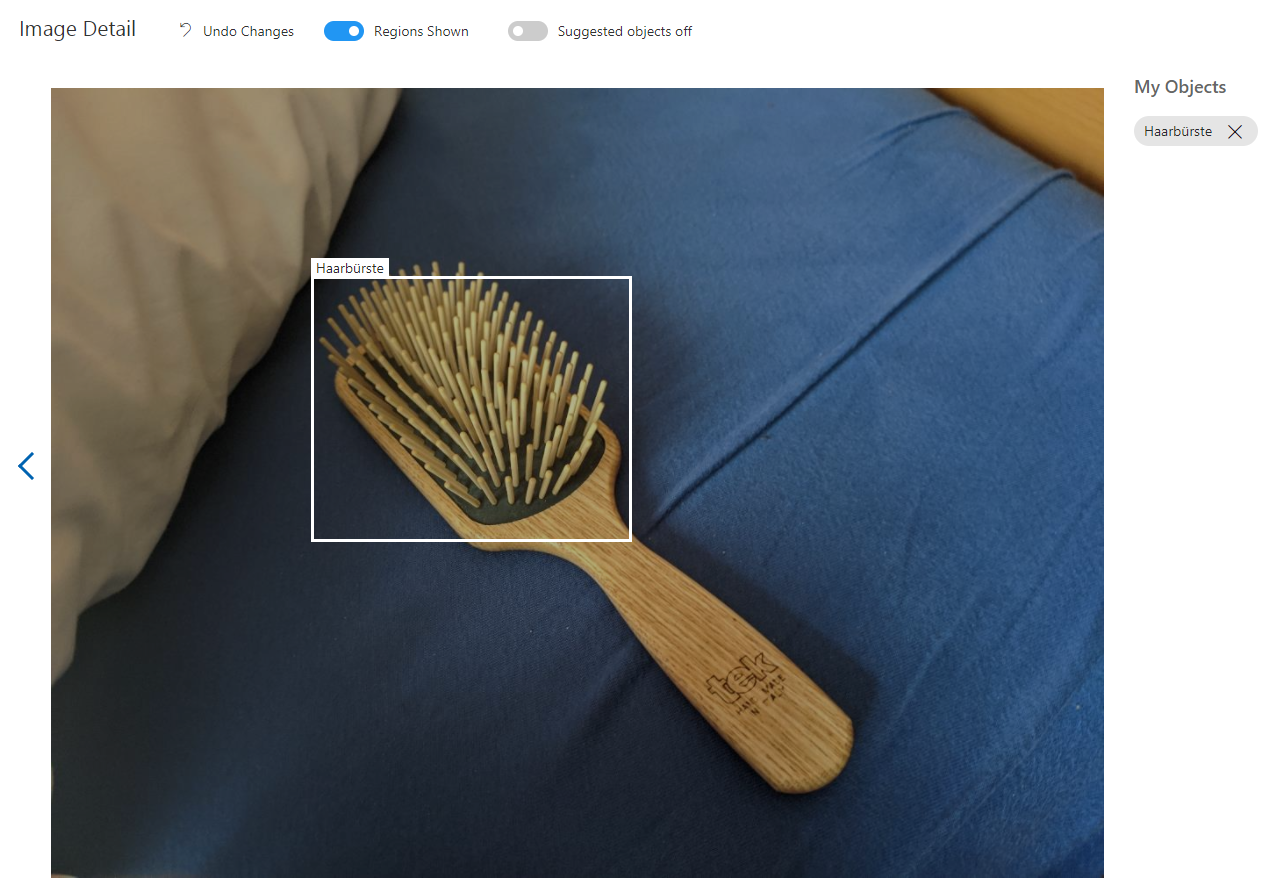
\includegraphics[width=1\textwidth]{images/trainingone.png}
	\caption[]{Trainingsbild für die Objekterkennung einer Haarbürste.}
	\label{img:trainingone}
\end{figure}

Für jede Objekt-Klasse müssen mindestens 15 Bilder hochgeladen werden, in denen der entsprechende Tag vorkommt. Nur kann kann der Trainingsprozess gestartet werden. Mit mehr Bildern in dem Trainingsset wird die Objekterkennung des Modells jedoch robuster. Azure empfehlt es mindestens 50 Bilder pro Tag zu verwenden. Wenn mit nur wenigen Bildern trainiert wird, haben die einzelnen gewählten Bilder einen sehr großen Einfluss auf das Modell.

Durch das Trainieren wird eine Iteration des Modells erzeugt. Diese Iteration kann verwendet werden, um Objekt Detection durchzuführen. Wird erneut der Trainingsprozess gestartet, wird eine weitere Iteration erstellt. Die Iterationen werden alle unter einen Projekt ID gespeichert.

Die Iterationen des Modells werden hinsichtlich ihrer Robustheit evaluiert. Für jede Objekt-Klasse werden drei Metriken angesetzt. 
\begin{itemize}
	\item Precision - die Wahrscheinlichkeit das ein gefundenen Objekt, tatsächlich der angegeben Klasse angehört. (Die Wahrscheinlichkeit das es kein false positive ist.)
	\item Recall - Aus einer Menge an Objekten die einer Klasse angehören, der Prozentsatz an Objekten, die das Model korrekt lokalisieren und klassifizieren konnte.
	\item a.p (Average Percision) - Eine Gesammtwertung für die Evaluierung basierend auf Percision und Recall. 
\end{itemize}

\begin{figure}[H]
	\centering
	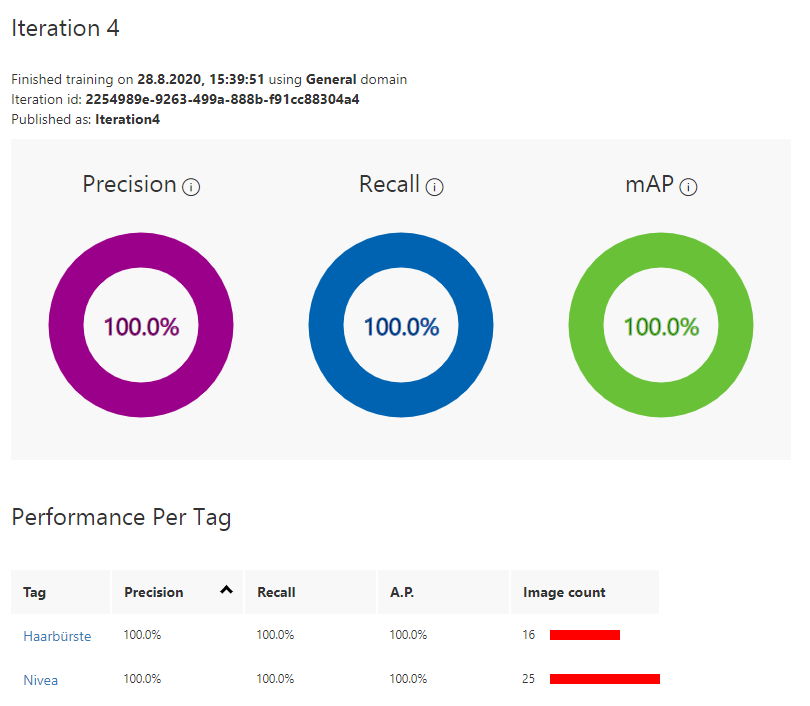
\includegraphics[width=1\textwidth]{images/trainingevaluation.png}
	\caption[]{Die Evaluierung des Modells}
	\label{img:trainineval}
\end{figure}

Mit einer Erstellen Iteration des Modells können Fotos auf Objekte untersucht werden. Ähnlich wie Azure Object Detection ist das Custom Modell durch eine REST-Api erreichbar. 
Der Endpoint beinhaltet die ID des Projektes, und die Nummer der Iteration, die verwendet werden soll.
In der Post Nachricht wird ein Authentifizierungsschlüssel und ein zu analysierendes Bild mitgeschickt.

Das Resultat der Analyse ist eine Json Datei. 
Der Aufbau des Resultats unterscheidet sich vom dem von Azure Object Detection leicht. Informationen über die Iteration, die für die Analyse verwendet wurde werden wiedergegeben. 

\begin{lstlisting}
{"id":"9cb0cc50-1dca-4b4a-b4d1-95d6bd25c352",
"project":"ac915246-5268-461f-bd11-cf0c1826d509",
"iteration":"2254989e-9263-499a-888b-f91cc88304a4",
"created":"2020-10-10T02:40:40.107Z",
"predictions":[{"probability":0.997380137,"tagId":"d390d34e-afc4-4ff4-8dcd-3ee8fe79cb8f","tagName":"Haarbürste","boundingBox":{"left":0.258805573,"top":0.226171583,"width":0.303168833,"height":0.329167157}},
{"probability":0.0141124222,"tagId":"d390d34e-afc4-4ff4-8dcd-3ee8fe79cb8f","tagName":"Haarbürste","boundingBox":{"left":0.542580664,"top":0.507969,"width":0.2195471,"height":0.3491398}},
{"probability":0.0116642443,"tagId":"263b3042-8958-4775-9a19-e2602d19c9b7","tagName":"Nivea","boundingBox":{"left":0.542580664,"top":0.507969,"width":0.2195471,"height":0.3491398}}]}
\end{lstlisting}

Die gefundenen Objekte werden in der Liste "predictions" aufgezählt. Die Objekt Klassen werden in "tagName" gespiechert. "probability" gibt die Konfidenz des Modells an, das das Objekt korrekt erkannt wurde. Die erkannten Objekte müssen bei nach ihrer probability gefiltert werden, da auch Objekte mit einer sehr niedrigen probability in in der Json Datei enthalten sind. 